%%%%%%%%%%%%%%%%%%%%%%% file tdp-draft.tex %%%%%%%%%%%%%%%%%%%%%%%%
%
% TDP Draft version 
% Created by Krit
%
%%%%%%%%%%%%%%%%%%%%%%%%%%%%%%%%%%%%%%%%%%%%%%%%%%%%%%%%%%%%%%%%%%%

\documentclass{llncs}

\usepackage{url}
\usepackage{amsmath}
\usepackage{array}
\usepackage{graphicx}

\newcommand{\dq}[1]{``#1''}
\newcommand{\dit}[1]{\dq{\textit{#1}}}
\newcommand{\md}[1]{\(#1\)}
\newcolumntype{C}[1]{>{\centering\let\newline\\\arraybackslash\hspace{0pt}}m{#1}}

\begin{document}

\title{SKUBA 2014 Team Description}
\author{Kanjanapan Sukvichai
\and Krit Chaiso
\and Thanakorn Panyapiang
\and Jaktip Yodsri
\and Suppawit Inhorm
\and Tachin Srisombat
\and Sutinai Tanalerkchai
}

\institute{ Faculty of Engineering, Kasetsart University\\
50 Ngamwongwan Rd, Ladyao, Bangkok, Thailand\\
\email{skuba2002@gmail.com}\\
\url{http://iml.cpe.ku.ac.th/skuba}
}

\maketitle

\begin{abstract}
This paper describe overview system of SKUBA, Robocup @Home robot team from Kasetsart University, in order to particiapte in Robocup @Home 2014. Our robot hardware doesn't have major change except the gripper that was redesinged to deal with object slip issue we encounter from previous Robocup. The research this year focus on speech recognition and object recogtion which are our main problems from last year competition. We'll mentiond about techniques and algorithms that we use to improve speech and object recognition ability in this document.
\end{abstract}

\section{Introduction}

SKUBA @home was established in 2011. In 2012, SKUBA @home made the first participation in Robocup Japan Open 2012 and made the way through finalist. Furthermore, SKUBA @home joined the World Robocup 2012 in Mexico and reach 2nd stage as we anticipated. Last year, we built the new robot by using mechanum wheel and proved that it was suitable for dynamic environment in Robocup Japan Open 2013, Tokyo. Lastly, we done well in \dq{Follow Me} task under World Robocup @home 2013 at Eindhoven.

During last year competition, we found two important problems that cause us perform lower than expectation. In disorganized environment, first problem is a tenacious robot with incorrect speech recognition. For instance, in \dq{Enduring General Purpose Service Robot} task, the robot repeatedly produce same error with same command. So, we decide to reduce this failure by propose new idea which will be described later. Second problem is unacceptable object recognition. In most tasks, robot have to grab the object to designated location. But our recognition system produces empty result then robot unable to start grabbing the object. For this reason, we abandon old recognition system and reimplement new system. New object recognition consists of machine learning and clustering technique which will be mentioned later.

The next section will explain about our robot mechanical and electrical design. In section 3, software architecture, new object recognition algorithm and voice recognition system are explained. Section 4 explain is about controlling robot movement, such as, motor control component and new manipulator handle component. Finally in the last section, we will present the conclusion.

\section{Robot Hardware}

The SKUBA@Home platform is designed as a three layeys. The first layer is the driving mechanism layer. This robot base consists of four 8'' mecanum wheels. Each mecanum wheel is driven by Maxon EC 45 flat (brushless motor, 70 watt) BLDC motor combined with planetary gearhead of 1:36 gear ratio. Because robot has to securely navigate, FPGA embedded is selected to control 4 motors simultaneously. The Hokuyo laser length finder is attached to the lower layer in order to obtain the environment information which will be used in localization and mapping algorithm. About this mecanum wheel is more mobility than the regular fixed wheel since it provides side movement. Therefore, the robot can easily avoid the obstacles and has more flexibility to maneuver to the messy environment. The second layer is the robot body. The robot body can be moved along vertical axis by using sliding bars which are driven by 70 watt DC windshield wiper motor. The robot head and arm are attached to this layer. The final layer is the robot head and arm. Robot head has two degrees of freedom neck which is similar to the human neck behavior. Kinect sensor, shotgun microphone and Logitech webcam is fixed to the top of the neck which can be used as the human-like head. High torque Dynamixel MX-106R servo, Dynamixel RX-64 servo, Dynamixel RX-28 servo and BLDC Maxon motor are used to construct the robot arm. For conducting BLDC motor, customized embedded is developed by using Arduino platform\cite{con_arm}. Robot arm has 6 degrees of freedom which can perform more complex tasks. Due to object slip from last gripper design, we proposed new gripper which more powerful and more sticky.

\begin{figure}
\centering
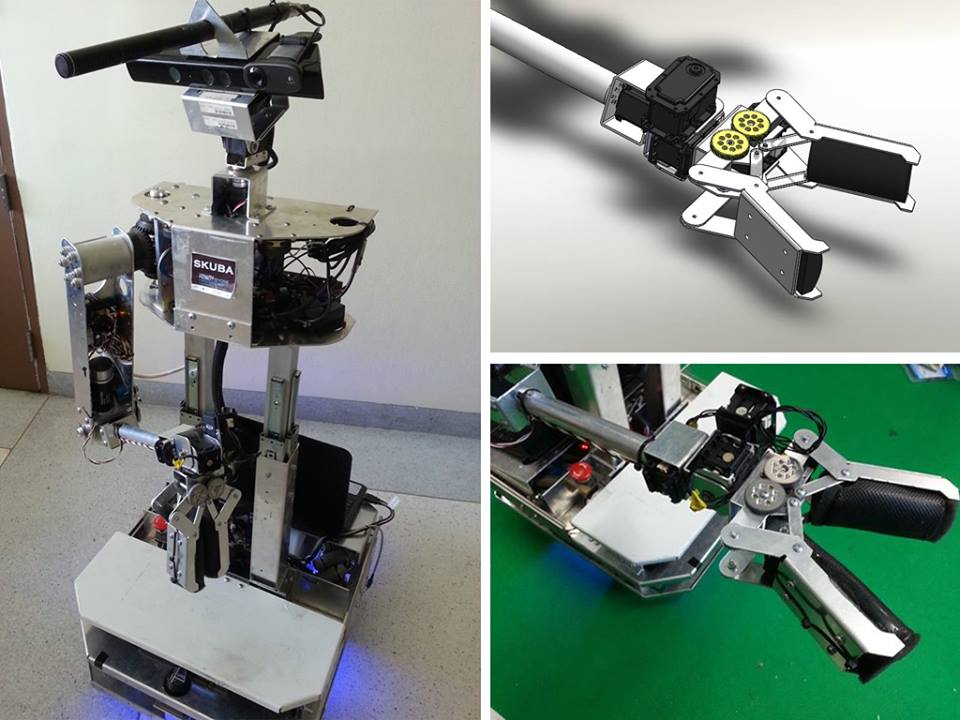
\includegraphics[height=6.2cm]{robot_hardware}
\caption{Robot hardware Left: The SKUBA@Home robot, Top Right: new gripper design, Bottom Right: actual gripper}
\label{fig:base}
\end{figure}

\section{Software Architecture}
Software system of our robot is divided into many modules with specific functionality, for example, object recognition module and planning module. The communication between modules is implemented by using Robot Operating System (ROS). The modules can be organized into three different layers:\textit{perception layer}, \textit{control layer} and \textit{decision layer}.

\textit{Perception layer} consist of modules about environmental understanding. Speech recognition, Object recognition and Localization, for instance. Modules in this layer collect data from sensors, i.e. laser range finder, microphone and Kinect, to perform higher-level algorithms in order to identify state of the environment. Output of this layer is intermediate data for \textit{decision layer}

\textit{Decision layer} control robot's behavior to solve complicated task. In this layer, decision is made base on user command and information from perception layer. User command is classified into three categories: \textit{question}, \textit{command} and \textit{informative}. \textit{Question} is a sentence which user expect to get a proper answer from robot. \textit{Command} is used when user want robot to perform any action, for example, \dq{Bring me a pringle} and \dq{Follow me}. When robot get an information, such as \dq{My name is Brian} and \dq{This is kitchen}, these sentences will be classified as the \textit{Informative command}.

When \textit{decision layer} send command to robot, \textit{Control layer} will interpret those commands into lower-level actions by using path planning algorithms. Furthermore, the layer also controls robot manipulator with precision.

\subsection{Voice System}

Speech recognition is implemented by using \textit{pocketsphinx} base on CMUSphinx, HMM-based speech recognition toolkit. Recognition process begin with spliting incoming audio into utterances and converted into sequence of words. The system require grammar and dictionary in order to do speech recognition. For specific situation, vocabulary corpus is created by combining between common phrases, such as \dq{My name is} and \dq{Bring me a} , and predefine name, e.g., \textit{Donna} and \textit{Pringle}. The tools used to make grammar and dictionary is the Sphinxbase which require a corpus(Java Speech Grammar Format) file as an input. To improve recognition accuracy, the system use feedback from users in case of the robot require user to verify their command, confirm their name, for instance. The recognition module use those user's feedback to modify and decrease probability of incorrect output. For speech synthesis, our robot use \textit{Flite}, speech synthesis engine developed at Carnegie Mellon University, which is a free text-to-speech engine. 

\subsection{Object Recognition}
    
To improve the precision of recognition module, localization approach is enhanced by using both RGB image and depth image together. First, depth information from OpenNI library is applied for extracting objects from the background scene using Euclidean Clustering Extraction\cite{ece}\cite{rudu.thesis}. Additionally, there are some explicit constrains, e.g., table plane boundary and manipulator work space limitation, to distinguish the cloud that is definitely not the interested object, such as, the object that are beneath the table. After computing the centroid of extracted point cloud, object's border is transformed using the focal length equation from 3D space to RGB domain. From object's border, the segmented image is obtained. In image domain, descriptors of the segmented image are extracted using Speeded-Up Robust Features(SURF), and can be classified by a recognition process.

Another developed process is a recognition process. Initially, the extracted descriptors are clustered using K-means clustering. Next, the histogram for each object is created by counting the number of descriptors in each cluster. Finally, the set of histograms are used as learning instance for SVM method which is supervised learning for classification the object category\cite{obj_rec}.

The performance of this approach gains us the higher efficiency of both localization and recognition. First of all, localization using depth information has the acceptable accuracy for scoping the object boundary from the background scene. Lastly, recognition process has a significance of accuracy in classification comparing to our old method. Finally, result of this module is shown in Fig.\ref{fig:object_recog}.

\begin{figure}
\centering
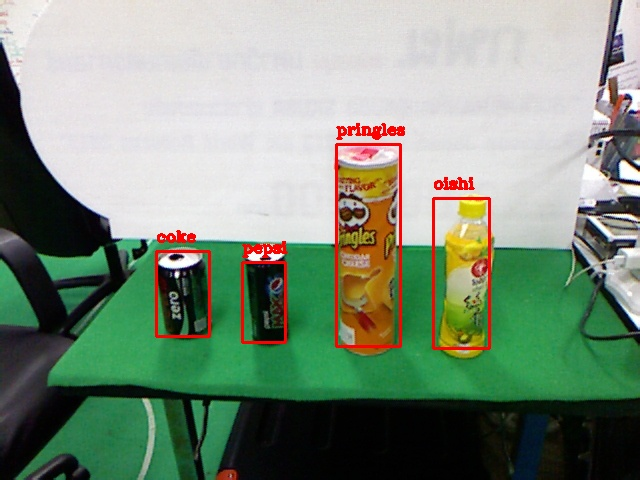
\includegraphics[height=6.2cm]{object_recognition_figure}
\caption{Result from object recognition module}
\label{fig:object_recog}
\end{figure}

\subsection{Gesture Recognition}

NITE library is included in OpenNI framework. It can retrieve motion gesture, e.g.., wave, circle, swipe, push and steady. Outputs from this library are hand position of all gesture detects. Moreover, it can be detect more than one gestures at a time. Therefore, we use NITE library in our gesture recognition module.

\subsection{Face Recognition}

Face recognition is basic ability for service robot to learn and classify human, such as, Serving meal and beverage. For this purpose, the robot has to memorize who is the owner of the order. Approach to face recognition, Elastic Bunch Graph Matching (EBGM) algorithm is chosen because of robustness to oriented variation\cite{face_reg}. First part of the algorithm is extracting face bunch graph by using predetermine facial landmarks. When receive the graph, each node is labelled by Gabor wavelet transform. In order to complete recognition task, it compares face graphs by using elastic matching. Finally, result of matching is clarified to be result of recognition module.

\subsection{People Detection and Tracking}

To pursue human, robot need two important functions which is human detection and designated person tracking. People detection method use the RGB-D, point cloud, data as the input to acquire people position. Avoiding the problem of detection, such as, consolidation of small crowd and obstruction of body part, sub-clustering of people's head is applied as the representation of each detected person. For each detected person, people location from people detection method is passed to tracking method. This method is implemented based on likelihood data association, online classification using color appearance, and HOG-based motion tracking\cite{pp_detect}. After performing tracking method, sequences of all people position is obtained. Results of our people detection and tracking module is shown in Fig.\ref{fig:people_detection}.

\begin{figure}
\centering
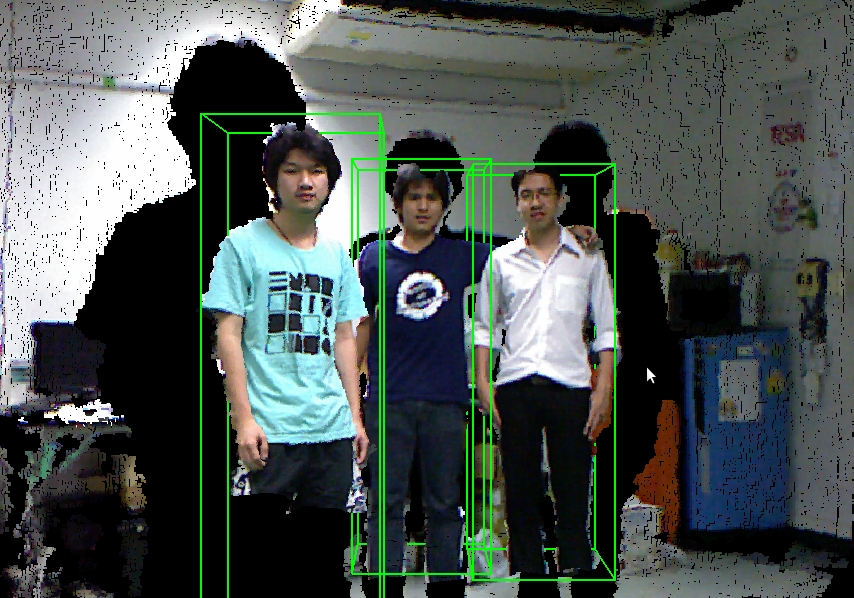
\includegraphics[height=5.2cm]{people_detection_figure}
\caption{Result from people detection and tracking}
\label{fig:people_detection}
\end{figure}

\section{Motion Control and Planning}

\subsection{Motor Control System}

Motor control system is composed of a collection of embedded controllers which executes the low level motor control loop, communication and debugging. First controller is base motor controller. The motor controller, increment quadrature decoder, PWM generation and onboard serial interfaces are implemented using FPGA. The PI controller is employed to achieve each wheel velocity. And the communication between controller and computer is established by using RS232. Furthermore, there is different controller to control arm motor. To interact with it, RS485 standard is selected and build in to the controller. For convenient usage, second controller also have PID-Torque control, torque limitation and orientation adjustment. 

\subsection{Localization and Path Planning}

Adaptive Monte Carlo Localization system (AMCL), provided by \textit{navigation} stack, is used for robot localization. To serve localization algorithm, Hokuyo laser length finder which acquires environmental data is attached to the robot. Additionally, the robot odometry information is also considered as one input information to localization algorithm. Another input is the known map which is statically or dynamically construct. From previously describe input, AMCL which is a particle filter localization system accurately estimates position and orientation of the robot.

The static and dynamic map is acquired by using \textit{hector\_mapping} package within \textit{hector\_slam} stack. This package requires only laser length finder data. To construct an occupancy grid map, it performs laser beam matching using Gauss-Newton approach\cite{hector_slam}. The comparison result between \textit{gmapping} and \textit{hector\_mapping} is shown in Fig.\ref{fig:hector}.

\begin{figure}
\centering
\caption{Comparison occupancy map between \textit{gmapping}(left) and \textit{hector\_mapping}(right)}
\label{fig:hector}
\end{figure}

To achieve path planning, there is \textit{move\_base} node in \textit{navigation} stack that is consist of two types of planning method. Begin with global planner, this method provides an effective path for robot to navigate through the known map. By using Dijkstra's algorithm, the result path is the shortest and acceptable. Then local planner method move to destination following designated path and avoid obstacles along the way. In order to move robot, local planner determine its velocity and orientation. This node directly send command to the robot.

\subsubsection{Odometry Estimation Module}

This module helps to minimize the mean square error of the non-perfect sensor measurement originated from wheel slippage, dynamic surrounded environment and IMU drift over time. Using the laser scanner to estimate the change of position by laser scan matching technique can solve the wheel slip problem while facing with high sensitivity and dynamic environment. Point-to-line distance Iterative Closed Point (ICP)\cite{icp1}\cite{icp2} method is used to be based algorithm for laser scan matching.

To perform estimation module, Kalman filter which consist of two steps is used. First, the Kalman's observation step calculates difference between output from last prediction and actual position which combine laser scan matching and wheels' speed together. Next, the Kalman's prediction step predicts new output by compensate error from previous step and IMU data\cite{odom}.

\subsubsection{Collision Avoidance Module}

This component ease the planning module to organize safety movement. By retrieve point cloud data from Kinect, this module projects each point to occupancy map. In order to avoid obstacles, path planner retrieve projection data and manage to construct smooth path. Due to unusual data, such as, ground plane and wall partition, planar elimination algorithm is applied. Result data from algorithm, for instance, table and chair, is projected and pass to planning module continuously\cite{avoid}.

\subsection{Manipulation Module}

For the manipulation system, two distinct methods are developed for serving various situation. First, grasping action method uses a shape of particular object as input. And it selects appropriate movement from predefine sequences of action and send command to robot arm. In generally, this method use for object which has a complicated shape. Another method is inverse kinematic method that receive the centroid of an object and directly control robot's manipulator. So, this method use with a simple object, e.g., can, box and bottle.

\section{Conclusion}

In this year, perception and manipulation are our main focuses. Especially, object recognition and voice system are developed to be more stable, precise and robust. We'll improve performance of dynamic localization and mapping as future work. We gained experiences from RoboCup@Home competition 2013 and discovered development idea. For Robocup@Home 2014 in Brazil, our robot are more autonomous and ready for engage in competition. We hope that our robot team will perform better in RoboCup than the previous year, and we are looking forward to sharing experiences with other great teams around the world.

\begin{thebibliography}{4}

\bibitem{con_arm} T. Ariyachartphadungkit and K. Sukvichai, Development of an Embedded BLDC motor controller using RS485 standard, 2013.

\bibitem{ece} S. Tuerker. Euclidean Cluster Extraction.\\
\url{http://pointclouds.org/documentation/tutorials/cluster_extraction.php}.

\bibitem{rudu.thesis} Radu B. Rusu, 
Semantic 3D Object Maps for Everyday Manipulation in Human Living Environments, Germany, 2009.

\bibitem{obj_rec} D. Schmitt and N. McCoy. Object Classification and Localization Using SURF Descriptors. 2011.

\bibitem{face_reg} L. Wiskott, J.M. Fellous, N. Kruger and C. Malsburg, Face Recognition by Elastic Bunch Graph Matching, IEEE Trans. PAMI, vol. 19, no. 7, pp. 775-780, 1997. 

\bibitem{pp_detect} M. Munaro, F. Basso and E. Menegatti. Tracking people within groups with RGB-D data. In Proceedings of the International Conference on Intelligent Robots and Systems (IROS) 2012, Vilamoura (Portugal), 2012.

\bibitem{hector_slam} S. Kohlbrecher and J. Meyer and O. von Stryk and U. Klingauf. A Flexible and Scalable SLAM System with Full 3D Motion Estimation, in Proc. IEEE International Symposium on Safety, Security and Rescue Robotics (SSRR), November, 2011.

\bibitem{icp1} A. Censi, An ICP variant using point-to-line metric, In Proceedings of the 2008 IEEE International Conference on Robotics and Automation (2008).

\bibitem{icp2} A. Censi, An accurate closed-form estimate of ICP's covariance, In Proceedings of the 2007 IEEE International Conference on Robotics and Automation (2007).

\bibitem{odom} B. Pholpoke and K. Sukvichai. Real Time People Tracking and Collision Avoidance using Sensors Fusion for an Indoor Omni-directional Wheels Mobile Robot, 2013.

\bibitem{avoid} T. Chaveekolakit and K. Sukvichai. Development of Ground Planar Segmentation algorithm using 3D Point Clouds Information from Kinect Depth Image Camera, 2013.

\end{thebibliography}

\end{document}
